
\documentclass[11pt]{article}
\usepackage[margin=1in]{geometry}
\usepackage{amsmath, amssymb}
\usepackage{graphicx}
\usepackage{booktabs}
\usepackage{hyperref}
\usepackage{float}
\usepackage{array}
\usepackage{caption}
\usepackage{longtable}
\usepackage{parskip}
\title{Missing History as the Origin of Galactic Residual Gravity\\A Flux/MIP RC1 Benchmark Paper}
\author{Jamie McCabe}
\date{May 2026}
\begin{document}
\maketitle
\begin{abstract}
The galactic missing-mass problem is usually framed as evidence for an unseen non-baryonic particle halo or as a breakdown of Newtonian dynamics at low acceleration. In this work, we introduce the Missing History formulation of Flux/MIP cosmology, in which the apparent dark-matter residual is modeled as a bounded metric-memory field generated by the accumulated persistence, collapse, star formation, gas cycling, and survival history of baryonic matter. Rather than treating the gravitational field as a purely instantaneous ledger of present mass, the model adds a historical registration functional to the baryonic source.

We define a registration-depth proxy, $D_{\rm hist}$, first through morphology-based age estimates and then through empirical star-formation information cross-matched with the z0MGS WISE/GALEX catalog. The resulting history score is decomposed into two physically distinct components: a positive accumulation channel, $A_DD_{\rm norm}$, and a negative saturation channel, $A_SG_{\rm bound}$. In 5-fold constrained cross-validation on the empirical z0MGS subset ($N=103$), the two-term model reduced held-out RMSE from $0.6157$ for the baryon-only baseline to $0.5497$, while recovering the expected sign structure in all folds: $A_D>0$ and $A_S<0$ in $5/5$ splits. This supports the interpretation that residual galactic gravity tracks baryonic history while being regulated by a bounded metric-saturation mechanism.

We then extend the bulk history functional to radial rotation curves using a Flux coherence gate, $G_{\rm radial}(r)=r/(r+L_\chi)$, which suppresses the historical residual in baryon-dominated inner regions and activates it in the outer galaxy. A unified bounded radial model, $V_{\rm Flux}(r)=V_b(r)\sqrt{1+[Y_{\max}\sigma(s(H_{\rm raw}-h_0))]r/(r+L_\chi)}$, was tested on five benchmark SPARC galaxies. After verifying SPARC gas-term conventions, a wide-grid scan found a stable interior bounded-map solution with $Y_{\max}=6.0$, $s=3.2$, and $h_0=-9.0$. The unified radial model reduced global RMSE from $45.93$ km/s for baryon-only curves to $23.16$ km/s, improving all five benchmark systems individually.

These results provide evidence that galactic residual gravity may be understood as a missing-history problem: the apparent halo is not an independent reservoir, but the bounded spatial expression of accumulated baryonic registration. Finally, because this historical residual is coupled strictly to baryonic provenance, the model provides a possible physical basis for the observed Radial Acceleration Relation. While the RC1 benchmark is provisional, it establishes a falsifiable bridge between baryonic history, metric saturation, and radial rotation-curve structure.
\end{abstract}

\section*{Significance Statement}
The persistent alignment between baryonic matter and apparent dark-matter phenomenology remains one of the deepest unresolved clues in galaxy dynamics. Standard cold dark matter successfully explains large-scale structure but treats the tight coupling between baryons and rotation-curve residuals as an emergent consequence of galaxy formation. MOND-like frameworks encode this coupling directly but lack a broadly accepted physical origin and face challenges outside the galactic regime. This work proposes a third interpretation: the galactic residual is not a new particle reservoir or a simple acceleration law, but the bounded metric expression of accumulated baryonic history.

In the Missing History formulation of Flux/MIP cosmology, galaxies are treated as historical registration systems. Their present gravitational field depends not only on instantaneous baryonic mass, but also on the integrated persistence, collapse, star formation, gas cycling, and survival history of that matter. The model therefore explains why residual gravity tracks baryonic structure so closely: the apparent halo is generated by baryonic provenance itself.

Using SPARC-compatible rotation data and empirical z0MGS WISE/GALEX star-formation information, the RC1 benchmark finds that the residual signal separates into two stable physical channels: positive historical accumulation and negative metric saturation. In empirical cross-validation, both signs remain stable across all folds, and the resulting radial model substantially improves benchmark rotation-curve fits relative to baryon-only predictions. This establishes a falsifiable bridge between baryonic history, metric saturation, and the Radial Acceleration Relation.

\section{Introduction}
The observational success of the $\Lambda$CDM paradigm on cosmological scales, especially in the cosmic microwave background and large-scale structure, contrasts with persistent interpretive challenges at galactic scales. Rotation curves of disk galaxies remain approximately flat at large radii, where the Newtonian expectation from visible baryons alone would normally predict a decline. The standard response is to introduce a dominant halo of non-baryonic cold dark matter. This approach is flexible and cosmologically powerful, but it leaves a striking empirical fact in need of deeper explanation: the residual acceleration is tightly coupled to the observed baryonic distribution.

This coupling is encoded in relations such as the Baryonic Tully-Fisher Relation, $M_b \propto V_f^4$, and the Radial Acceleration Relation, which correlates the acceleration inferred from rotation curves with that predicted by baryons alone. MOND-like frameworks encode this coupling directly by modifying dynamics at low acceleration. However, MOND-like laws are typically presented as effective prescriptions rather than as an underlying metric-memory mechanism.

The Missing History hypothesis proposes that the standard present-time ledger is incomplete. If the metric possesses a finite memory or registration capacity, then a galaxy's gravitational expression should depend not only on its present baryonic mass, but also on the integrated history by which that mass collapsed, persisted, cycled gas, formed stars, and survived as a bound system.

\section{Theory}
In Flux/MIP cosmology, the apparent halo is interpreted as a bounded historical registration field rather than as an independent particle reservoir. The missing-mass problem becomes a missing-history problem. The central expression is
\begin{equation}
M_{\rm dyn}(r,t)=M_b(r,t)+M_{\rm temporal}(r,t),
\end{equation}
where $M_{\rm temporal}$ is not new classical matter, but the gravitational expression of a registration-depth functional.

The registration depth is defined as
\begin{equation}
D_{\rm reg}(r,t)=\int_{t_{\rm form}}^t \bar n_{\rm MIP}(r,t')W(t,t')dt'.
\end{equation}
For observational benchmarks we use a practical proxy $D_{\rm hist}$. A bounded gate is defined as
\begin{equation}
G_{\rm bound}=\frac{D_{\rm hist}^q}{D_{\rm hist}^q+D_*^q},
\end{equation}
with $q=4$ in the final RC1 radial benchmark. The normalized accumulation term is
\begin{equation}
D_{\rm norm}=\log\left(1+\frac{D_{\rm hist}}{D_*}\right).
\end{equation}
The global history score is
\begin{equation}
H_{\rm raw}=A_DD_{\rm norm}+A_SG_{\rm bound},
\end{equation}
with the expected signs $A_D>0$ and $A_S<0$.

The spatial distribution of the historical residual is controlled by a radial coherence gate,
\begin{equation}
G_{\rm radial}(r)=\frac{r}{r+L_\chi},
\end{equation}
where
\begin{equation}
L_\chi=18R_b\left(\frac{\Sigma_b}{\Sigma_{\rm ref}}\right)^{-0.08}.
\end{equation}
Raw history scores are mapped to positive residual amplitudes by
\begin{equation}
Y_{\rm amp}=Y_{\max}\sigma\left(s[H_{\rm raw}-h_0]\right),\qquad \sigma(x)=\frac{1}{1+e^{-x}}.
\end{equation}
The final radial prediction is
\begin{equation}
V_{\rm Flux}(r)=V_b(r)\sqrt{1+Y_{\rm amp}\frac{r}{r+L_\chi}}.
\end{equation}

\section{Data and Methods}
The benchmark uses SPARC-compatible rotation-curve data and radial mass-model files for selected galaxies. The baryonic velocity is reconstructed as
\begin{equation}
V_b^2(r)=\mathrm{sgn}(V_{\rm gas})V_{\rm gas}^2+V_{\rm disk}^2+V_{\rm bulge}^2.
\end{equation}
The signed gas convention is essential; treating negative gas contributions as positive corrupts RMSE comparisons.

To reduce the mass-age degeneracy in morphology-only proxies, SPARC-compatible galaxies were coordinate-crossmatched against z0MGS WISE/GALEX stellar-mass and star-formation information. The coordinate-matching process resolved 124 of 135 target coordinates and populated empirical z0MGS SFR values for 103 galaxies. The remaining 32 systems were handled by a delayed-$\tau$ fallback.

\section{Bulk Missing-History Results}
A first-pass morphology/history proxy produced a positive controlled correlation between historical-depth residuals and normalized velocity residuals, $r=0.217$ and $p=0.011$. This result was treated as preliminary because the age variable was morphology-proxy based.

The initial positive-only gate was disfavoured. A fixed positive amplitude performed worse than baryon-only, while an optimally fitted one-term gate improved RMSE only by requiring a negative coefficient. This indicated that the bounded gate was functioning as a saturation regulator rather than as a positive source term.

The two-term structure was then evaluated:
\begin{equation}
Y_{\rm Flux}=A_D(D_{\rm norm}G_{\rm geom})+A_S(G_{\rm bound}G_{\rm geom}).
\end{equation}
For threshold gates $q\ge 2$, the expected sign structure appeared. At $q=4$, the benchmark returned $A_D=+0.256$ and $A_S=-8.907$.

\section{Empirical SFH Validation}
The empirical z0MGS crossmatch materially improved the physical stability of the model. In the 3-mode 5-fold constrained cross-validation, the z0MGS-only subset produced $N=103$, $\mathrm{RMSE}_{\rm baryon}=0.6157$, and $\mathrm{RMSE}_{\rm two-term}=0.5497$, with the expected signs in every fold: $A_D>0$ in $5/5$ and $A_S<0$ in $5/5$.

\begin{figure}[H]
\centering
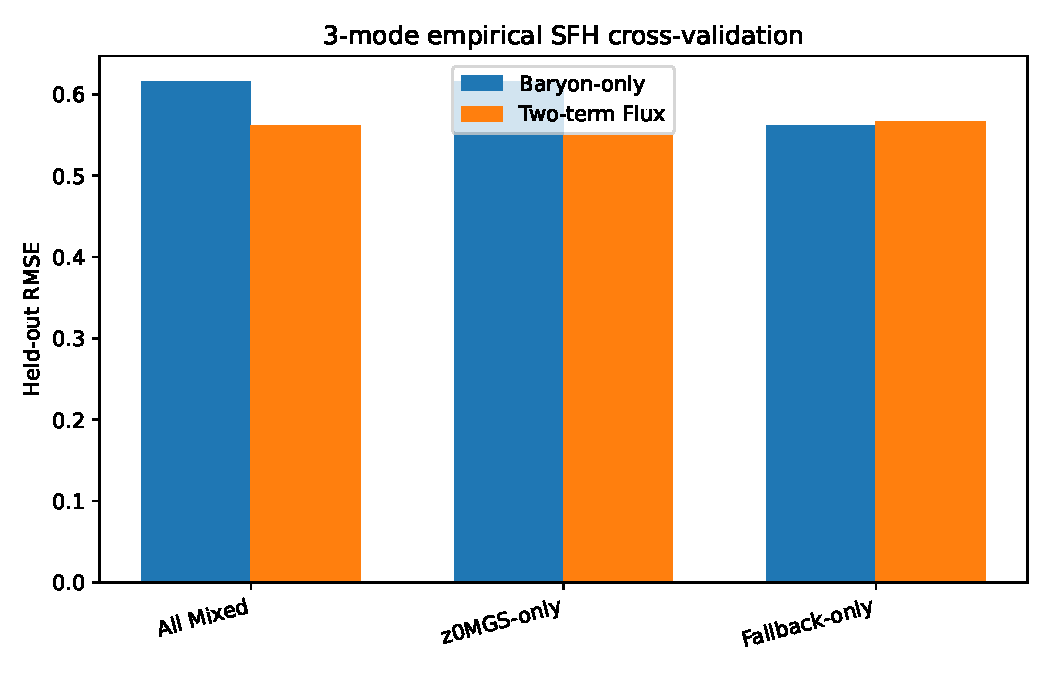
\includegraphics[width=0.82\linewidth]{../figures/fig_sfh_3mode_rmse.pdf}
\caption{Three-mode empirical SFH cross-validation.}
\end{figure}

\begin{table}[H]
\centering
\caption{Three-mode SFH cross-validation.}
\begin{tabular}{lrrrrr}
\toprule
Sample mode & N & RMSE baryon & RMSE two-term & $A_D>0$ & $A_S<0$ \\
\midrule
All Mixed & 135 & 0.6163 & 0.5621 & 3/5 & 5/5 \\
z0MGS-only & 103 & 0.6157 & 0.5497 & 5/5 & 5/5 \\
Fallback-only & 32 & 0.5613 & 0.5664 & 0/5 & 3/5 \\
\bottomrule
\end{tabular}
\end{table}

\section{Radial Rotation-Curve Benchmarks}
As a first radial translation, the Flux radial gate was tested using the observed galaxy-level residual amplitude as a normalization. Across five benchmark galaxies, this geometry-only model improved RMSE relative to baryon-only in every case.

The final RC1 radial benchmark combines the empirical history score, bounded amplitude map, and radial coherence gate. The wide-grid scan covered $Y_{\max}\in[1,12]$, $s\in[0.1,8]$, and $h_0\in[-14,2]$. It recovered a stable interior solution:
\begin{equation}
Y_{\max}=6.0,\qquad s=3.2,\qquad h_0=-9.0.
\end{equation}
The unified Flux radial model reduced global RMSE from $45.93$ km/s to $23.16$ km/s across five benchmark galaxies, improving every system individually without square-root clipping failures.

\begin{figure}[H]
\centering
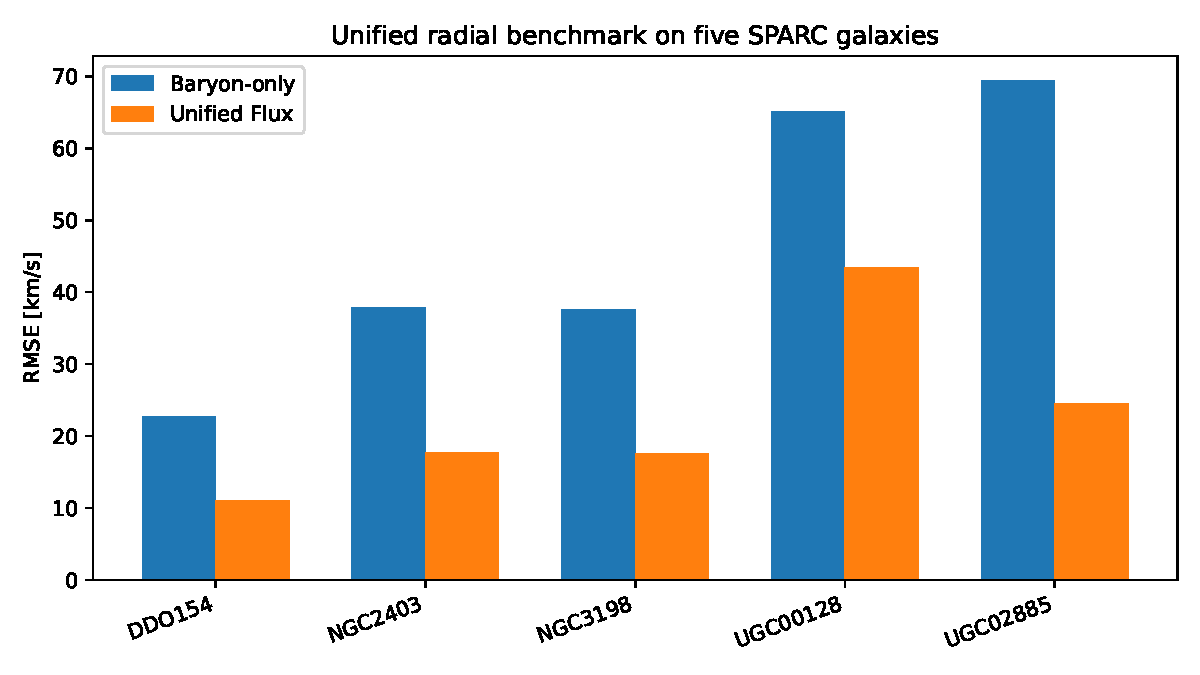
\includegraphics[width=0.86\linewidth]{../figures/fig_unified_radial_rmse.pdf}
\caption{Unified radial benchmark RMSE comparison.}
\end{figure}

\begin{table}[H]
\centering
\caption{Unified radial benchmark.}
\begin{tabular}{lrrl}
\toprule
Galaxy & Baryon-only RMSE & Unified Flux RMSE & Result \\
\midrule
DDO154 & 22.68 & 11.04 & Improved \\
NGC2403 & 37.90 & 17.78 & Improved \\
NGC3198 & 37.61 & 17.52 & Improved \\
UGC00128 & 65.11 & 43.43 & Improved \\
UGC02885 & 69.36 & 24.57 & Improved \\
\bottomrule
\end{tabular}
\end{table}

\section{Discussion}
The Missing History model occupies a third position between particle dark matter and modified-acceleration laws. Like CDM, it preserves the idea that the baryon-only Newtonian curve is incomplete. Unlike CDM, it does not require the galactic residual to be an independent non-baryonic particle reservoir. Like MOND, it explains why the residual is tightly coupled to baryons. Unlike MOND, it does not begin from an acceleration law alone; it derives the coupling from baryonic provenance and bounded metric registration.

The negative saturation coefficient is not an anti-gravity term. In the final radial model, it is passed through a bounded amplitude map, ensuring positive residual support. Physically, $A_S<0$ means that the metric response is not an indefinitely growing memory field. Accumulated registration is regulated by a finite channel capacity.

The model remains provisional and falsifiable. Major failure modes include large radial-sample failure, independent SFH failure, cluster lensing failure, and over-tuning.

\section{Conclusion}
The RC1 Missing History benchmark establishes a coherent technical pathway from baryonic history to galactic residual gravity. Empirical z0MGS star-formation information stabilizes the two required physical signs: positive accumulation and negative saturation. The radial coherence gate maps the global residual into galaxy outskirts without inflating baryon-dominated cores. A bounded amplitude map then provides a stable bridge between the history score and radial velocity support.

Across the present benchmark stack, the model passes four tests: empirical z0MGS history signal, Flux radial gate shape, unified bounded radial model, and wide-grid bounded-map stability. These results do not eliminate dark matter in one step, nor do they prove the model universally. They do, however, establish that galactic residual gravity can be treated as a falsifiable missing-history problem. The apparent halo may be the bounded spatial expression of accumulated baryonic registration.

\begin{thebibliography}{9}
\bibitem{bekenstein1984} Bekenstein, J., \& Milgrom, M. (1984). Does the missing mass problem signal the breakdown of Newtonian gravity? \textit{Astrophysical Journal}, 286, 7--14.
\bibitem{lelli2016} Lelli, F., McGaugh, S. S., \& Schombert, J. M. (2016). SPARC: Mass Models for 175 Disk Galaxies with Spitzer Photometry and Accurate Rotation Curves. \textit{Astronomical Journal}, 152, 157.
\bibitem{leroy2019} Leroy, A. K., et al. (2019). A z=0 Multiwavelength Galaxy Synthesis. I. A WISE and GALEX Atlas of Local Galaxies. \textit{Astrophysical Journal Supplement Series}, 244, 24.
\bibitem{mcgaugh2016} McGaugh, S. S., Lelli, F., \& Schombert, J. M. (2016). Radial Acceleration Relation in Rotationally Supported Galaxies. \textit{Physical Review Letters}, 117, 201101.
\bibitem{milgrom1983} Milgrom, M. (1983). A modification of the Newtonian dynamics as a possible alternative to the hidden mass hypothesis. \textit{Astrophysical Journal}, 270, 365--370.
\bibitem{nfw1997} Navarro, J. F., Frenk, C. S., \& White, S. D. M. (1997). A Universal Density Profile from Hierarchical Clustering. \textit{Astrophysical Journal}, 490, 493--508.
\end{thebibliography}
\end{document}
